\begin{multicols}{3}[\section{Bluetooth 3.0}]

\rhead{Autor: Johannes Hill}
\lfoot{Letzte Bearbeitung: 16.04.2016}
\newrefsegment

\begin{boxedminipage}{\linewidth}
\begin{tabular}{p{2,1 cm}p{2.7 cm}}
\textbf{Steckbrief}& \\
\end{tabular}
\begin{tabular}{p{1,5 cm}|p{3.3 cm}}
      Einsatz seit & April 2009\\
      \hline
      Frequenz"-bereich  & \SI{2,402}{\giga\hertz}~-~\SI{2,480}{\giga\hertz}\\
      \hline
      Datenrate & \SI{3}{Mbit/s} ohne L2CAP \SI{24}{Mbit/s} mit L2CAP\\
      \hline
      Verbreitung & Weltweit\\
      \hline
      Reichweite & \SI{10}{\metre}~-~\SI{100}{\metre}\\
\end{tabular}
\end{boxedminipage}
\par
%Source http://www.fh-bingen.de/fileadmin/user_upload/Lehrende/Kilsch_Dieter/internet/projekte/TedoSchStiUnits.pdf -> Seite 9 findet ihr alle verwendbaren Einheiten, wie:
%\SI{Zahl}{\mega\hertz} oder \SI{Zahl}{\mili\metre}
%Ich weiß ehrlich gesagt nicht welche Einheiten ihr im Text genau braucht, aber in dem Dokument und mit obigen Beispiel sollte es umsetzbar ein.
\subsection*{Überblick}

\begin{wrapfigure}{r}{0.4\linewidth}
  \vspace{-20pt}
  \begin{center}
  	\hspace{-20pt}
    
\includegraphics[width=0.7\linewidth]{Kapitel/Bluetooth3.0/Grafiken/logo.jpg}
  \end{center}
  \vspace{-15pt}
\end{wrapfigure}

Heutzutage haben elektronische Geräte dank der Miniaturisierung Einzug in das alltägliche Leben gefunden. Mit Bluetooth 3.0, auch bekannt unter dem Code Namen Seattle, können Geräte drahtlos und ohne direkte sichtbare Verbindung miteinander kommunizieren. Darüber hinaus sind die einzelnen Bluetooth Versionen aufgrund von Bluetooth Standard- und Interoperabilitätstest abwärtskompatibel. Das bedeutet, dass Bluetooth 2.1 + EDR Geräte problemlos mit Bluetooth 3.0 Geräten kommunizieren können~\cite{bluetooth3.0.1}. 

Bei der Entwicklung der Bluetooth 3.0 Spezifikation wurde vor allem das Ziel verfolgt, eine wesentliche Steigerung der Datenrate zu realisieren. Sein Vorgänger, sprich Bluetooth 2.1 + EDR, konnte nur eine Datenrate von 3 Mbit/s aufweisen. Damit eine Steigerung der Datenrate verzeichnet werden konnte, war es notwendig eine andere physikalische Schicht zu implementieren. Entsprechende Planungen begannen im Jahr 2006, wobei zwei Ansätze verfolgt wurden: 
\begin{itemize}
	\item Ultra-Wideband  und
	\item IEE 802.11.
\end{itemize} 
Das Ultra-Wideband, das durch die WiMedia Alliance entwickelt wurde, klang anfangs vielversprechend, da es einen geringen Stromverbrauch bei der Byte-Übertragung aufwies. Jedoch war der Stromverbrauch von Ultra-Wideband Controllern zu hoch für mobile Geräte, weshalb dieser Ansatz nicht weiter verfolgt wurde~\cite{bluetooth3.0.2}. 

Die Bluetooth Special Interest Group (SIG) hingegen, legte ihren Fokus den IEEE 802.11. Sie definierte für die Bluetooth 3.0 + HS (High Speed) Spezifikation einen generischen Abstraktions-Layer A2MP (\textbf{A}lternate MAC/PHY \textbf{M}anager \textbf{P}rotocol) für den AMP (\textbf{A}lternate \textbf{M}AC/\textbf{P}HY) und einen 802.11 PAL (\textbf{P}rotocol \textbf{A}dapatation \textbf{L}ayer) für den IEEE 802.11-2007 Standard. Diese Spezifikation ermöglicht zwei Systemvarianten. Bluetooth 3.0 (ohne HS) und Bluetooth 3.0 + HS~\cite{bluetooth3.0.2}.   

\subsection*{Technische Erläuterungen}
Bluetooth verwendet zwei unterschiedliche Kommunikationstypen. Dies ist zum einen die leitungsvermittelte synchrone Kommunikation (SCO) und zum anderen die paketvermittelte asynchrone Kommunikation (ACL). SCO wird nur zur Übertragung von Sprachdaten verwendet. Dementsprechend findet ACL seine Anwendung bei der restlichen Datenübertragung via Bluetooth~\cite{bluetooth3.0.4}.

Bei der Datenübertragung über den Bluetooth Kanal ist die maximale Datenrate auf die Endgeräte, die direkt miteinander kommunizieren, aufgeteilt. Die Datenrate eines Teilnehmers ist daher von folgenden Faktoren abhängig:
\begin{itemize}
	\item Anzahl der Endgeräte, die untereinander gleichzeitig Daten austauschen.
	\item Aktivität anderer Endgeräte.
\end{itemize}
Da Bluetooth das \SI{2,4}{\giga\hertz} Frequenzband nicht alleine verwendet, sondern dieses mit anderen Funktechnologien teilt, sendet Bluetooth nicht mit auf einer festen Frequenz, sondern variiert diese nach jedem Paket. Das angewendete Verfahren wird auch Frequency Hopping Spread Spectrum (FHSS) genannt. Sollte bei der Übertragung eines Pakets über den Kanal ein Fehler auftreten, werden die Daten automatisch erneut übertragen. Weiterhin gilt, dass ein Kanal in sogenannte Zeitschlitze (Slots) der Länge $625\mu$ unterteilt ist~\cite{bluetooth3.0.1}.

Um mehrere Bluetooth Verbindungen (Piconetze) zu garantieren, verwendet jedes Piconetz eine unterschiedliche Hopping-Sequenz. Im \SI{2,4}{\giga\hertz} Frequenzband können 79 Känale angeboten werden~\cite{bluetooth3.0.3}.

\subsubsection*{Klassen und Reichweite}
Bluetooth wurde hauptsächlich für portable Handhelds konzipiert, weshalb der Standard drei verschiedene Sendeleistungen spezifiziert. Entsprechend werden Endgeräte den einzelnen Leistungsklassen zugewiesen. Mobiltelefone sind beispielsweise der Leistungsklasse 3 zugeordnet~\cite{bluetooth3.0.5}. \\

\noindent
\begin{boxedminipage}{\linewidth}
\begin{tabular}{p{1,3cm} | p{1,5cm} | p{1,5cm}}
      \textbf{Klasse} & \textbf{Max. Leistung} & \textbf{Reichweite} \\
      \hline
      Klasse 1 & 100 mW & ca. 100m \\
      \hline
      Klasse 2 & 2,5 mW & ca. 50m \\
      \hline
      Klasse 3 & 1 mW & ca. 10m \\
\end{tabular}
\end{boxedminipage}

\subsubsection*{Piconetze}
Unter einem Piconetz versteht man eine Menge von miteinander kommunizierenden Bluetooth-Geräten. Verknüpft man Piconetze über Bluetooth-Geräte, können diese zu einem sogenannten Scatternetz zusammengefasst werden (siehe Abb. \ref{fig:Piconetze})~\cite{bluetooth3.0.3}.


\begin{Figure}
\begin{center}
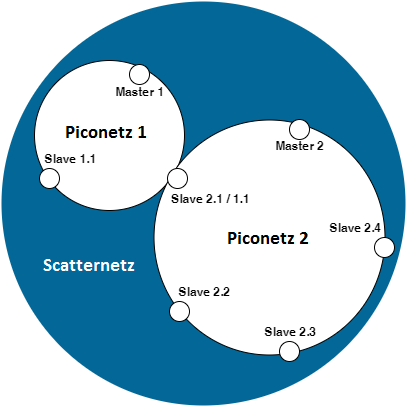
\includegraphics[scale=0.4]{Kapitel/Bluetooth3.0/Grafiken/piconetze.png}
\end{center}

\captionof{figure}{Piconetze und Scatternetze}
\label{fig:Piconetze}
\end{Figure}

\noindent
Piconetze sind aufgeteilt in ein Master- und bis zu sieben Slave Endgeräte. Dabei kann jedes Endgerät Master oder Slave eines Piconetzes sein. Dem Master ist die Aufgabe der Kontrolle des Kanals zugeschrieben, d.h. er entscheidet wer zu welchem Zeitpunkt Datenpakete über den Kanal verschicken darf. Damit dem Slave Endgeräte Senderechte zugewiesen werden kann, schickt ihm der Master ein entsprechendes Datenpaket. Diese Rechte werden dem Slave nach 5 Zeitslots wieder entzogen und der Master entscheidet, ob er ihm diese wieder gewährt. Darüber hinaus kann ein Slave keine weiteren Verbindungen zu anderen Geräten aufbauen, da für ihn nicht absehbar ist, wann Datenpakete vom Master eingehen. Um diese Problematik zu lösen, besteht die Möglichkeit, dass Master und Slave die Rollen tauschen~\cite{bluetooth3.0.1}.

Damit unterschiedliche Piconetze an einem Standort betrieben werden können, kommt das Verfahren des Frequency Hopping zum Einsatz. Dieses berechnet aus der Hardwareadresse des Endgerätes, das eine Verbindung zu anderen Endgeräten aufbauen möchte, die entsprechende Frequency Hopping Sequenz (siehe Abb. \ref{fig:SequenceHopping})~\cite{bluetooth3.0.3}.

\begin{Figure}
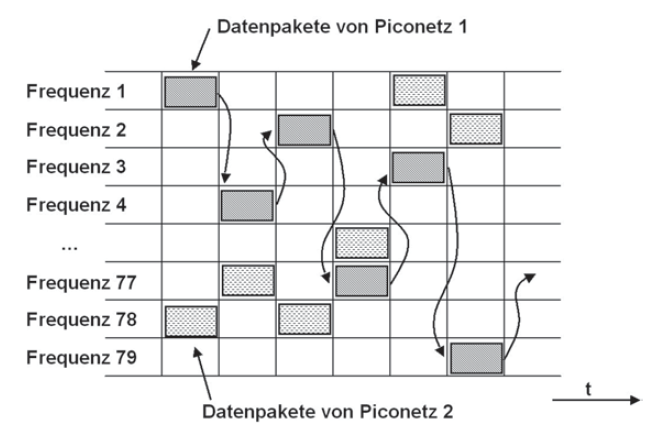
\includegraphics[width=\linewidth]{Kapitel/Bluetooth3.0/Grafiken/frequencehopping.png}
\captionof{figure}{Mehrer Piconetze am gleichen Ort durch Hop-Sequenzen~\cite{bluetooth3.0.1}}
\label{fig:SequenceHopping}
\end{Figure}

\subsubsection*{Der Bluetooth Protokoll Stack}
Grundlage für den Bluetooth Protokoll Stack bildet die ISO-OSI Schichtung (siehe Abb. \ref{fig:ProtokollStack}).Im Folgendem werden die Schichten zwei bis sechs vorgestellt und beschrieben.

\begin{Figure}
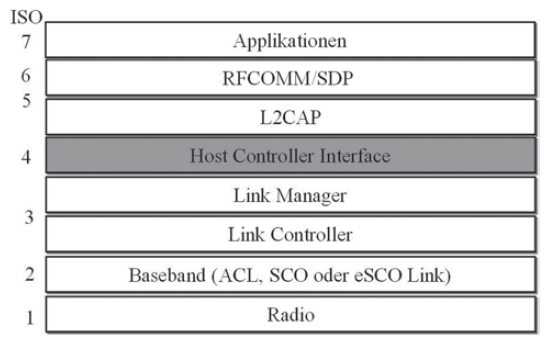
\includegraphics[width=\linewidth]{Kapitel/Bluetooth3.0/Grafiken/Protokoll_Stack.png}
\captionof{figure}{Der Bluetooth Protokoll Stack ~\cite{bluetooth3.0.1}} 
\label{fig:ProtokollStack}
\end{Figure}

\noindent
Der Base Layer übernimmt typische Aufgaben einer Layer 2 Schicht, wie z.B. dem Framing von Datenpaketen. Entsprechende Frametypen wurden bereits unter den Kürzeln SCO und ACL vorgestellt~\cite{bluetooth3.0.1}. 

Für den Aufbau, Erhalt und den korrekten Abbau von Verbindungen ist der Link Controller \hspace{1px} zuständig. Zu \hspace{1px} seinen \hspace{1px} weiteren \hspace{1px} Aufgaben zählen das Steuern der Funkkanäle, Frequenzwechsel und Funkverbindungen, sowie die Fehlerkorrektur (Forward Error Correction FEC) bei der Datenübertragung~\cite{bluetooth3.0.3}.

\end{multicols}
\newpage
\section*{Historische Entwicklung}
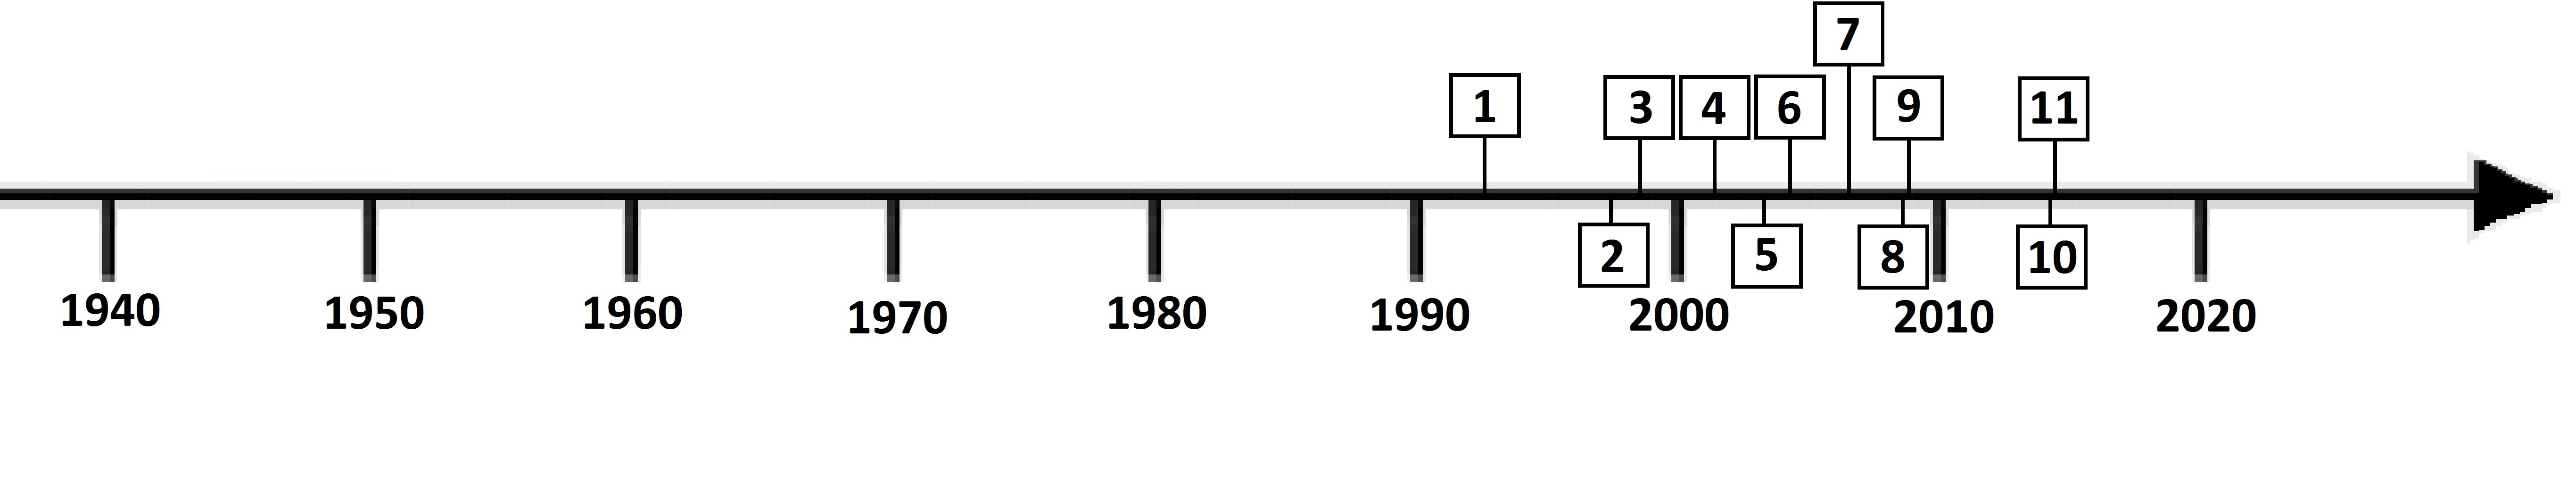
\includegraphics[width=\textwidth]{Kapitel/Bluetooth3.0/Grafiken/Zeitstrahl}
\par
\noindent

\vspace{-0.3cm}
\begin{tabular}{|p{1 cm}|p{3 cm}|p{13.55 cm}|}
	\hline
	Nummer & Datum & Information \\
	\hline
	1 & August 1993 & Gründung der Infrared Data Association (IrDA) mit dem Ziel ein einheitliches Protokoll für Datenübertragung über Infrarot bereitzustellen.\\
	\hline
	2 & 1998 & Gründung der Bluetooth Special Interest Group (SIG) durch die Firmen Ericsson, Nokia, IBM, Toshiba und Intel zur Ausarbeitung eines Standards, der verbindliche Spezifikationen festlegte.\\
	\hline
	3 & Juli 1999 & Bereitstellung der Spezifikation Bluetooth 1.0 (Juli) und Bluetooth 1.0b (Dezember).\\
	\hline
	4 & Februar 2001 & Bereitstellung der Spezifikation Bluetooth 1.1.\\
	\hline
	5 & November 2003 & Bereitstellung der Spezifikation Bluetooth 1.2.\\
	\hline
	6 & November 2004 & Bereitstellung der Spezifikation Bluetooth 2.0 + EDR.\\
	\hline
	7 & August 2007 & Bereitstellung der Spezifikation Bluetooth 2.1 + EDR.\\
	\hline
	\textbf{8} & \textbf{April 2009} & \textbf{Bereitstellung der Spezifikation Bluetooth 3.0 + HS}.\\
	\hline
	9 & Dezember 2009 & Bereitstellung der Spezifikation Bluetooth 4.0.\\
	\hline
	10 & Dezember 2013 & Bereitstellung der Spezifikation Bluetooth 4.1.\\
	\hline
	11 & Dezember 2014 & Bereitstellung der Spezifikation Bluetooth 4.2.\\
	\hline
\end{tabular}
\begin{multicols}{3}

Der Link Manager ist für die Einrichtung und Aufrechterhaltung von Verbindungen zuständig. Dazu wird das Link Manager Protocol (LMP) eingesetzt, welches ebenfalls Sicherheit, Identifikation und Verbindungskontrolle garantieren soll~\cite{bluetooth3.0.3}.

Mit dem Host Controller Interface (HCI) verfolgt man das Ziel, Endgeräte und Bluetooth Chip physikalisch voneinander zu trennen. Zu seiner Aufgabe zählt es, Daten und Kommandos für den Link Manager in definierten Kommandos und Nachrichtenpaketen zwischen Endgerät und Bluetooth Chip (Controller) zu übertragen~\cite{bluetooth3.0.1}.

Das Logical Link Control und Adaption Protocol (L2CAP) unterscheidet Protokolle von höheren Ebenen (z.B. RFCOMM, BNEP und SDP) und kann mehrere Verbindungen zu einem Gerät über eine physikalische ACL Verbindung multiplexen (siehe Abb. \ref{fig:l2cap}). Durch die Erweiterung des L2CAP in der Bluetooth Spezifikation 3.0 war es nun möglich den High Speed Kanal zu nutzen~\cite{bluetooth3.0.1}.

\begin{Figure}
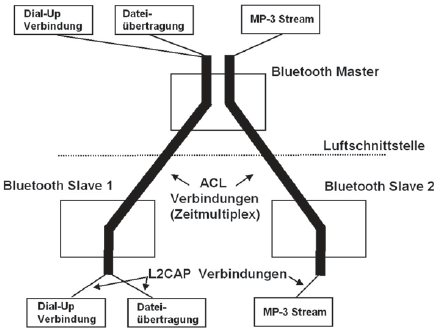
\includegraphics[width=\linewidth]{Kapitel/Bluetooth3.0/Grafiken/l2cap.png}
\captionof{figure}{Der Bluetooth Protokoll Stack~\cite{bluetooth3.0.1}}
\label{fig:l2cap}
\end{Figure} 

\noindent
Abschließend sollen das Service Discovery Protocol (SDP) und die Radio Frequency Comport Emulation (RFCOMM) betrachtet werden. SDP hat die Funktion, die für Anwendungen zur Verfügung stehenden Dienste ausfindig zu machen. RFCOMM hingegen stellt virtuelle serielle Schnittstellen für Dienste zur Verfügung und vereinfacht diesen dadurch die Datenübertragung ~\cite{bluetooth3.0.3}.

\subsubsection*{Bluetooth 3.0 Erneuerungen}
Mit der Bluetooth Spezifikation 3.0 wurde das Enhanced Power Control für ein effizienteres Energiemanagement eingeführt. Weiterhin implementierte man den High Speed (HS) Modus, der für den Verbindungsaufbau Bluetooth verwendet und für die Datenübertragung den Wi-Fi Kanal nutzt~\cite{bluetooth3.0.1}.

Die technische Umsetzung sah vor, den BR/EDR (\textbf{B}asic \textbf{R}ate/\textbf{E}nhanced \textbf{D}ata \textbf{R}ate) Controller von Bluetooth 1.X/2.X um einen oder mehrere AMP (Alternate MAC/PHY) und einen ULP (Ultra Low Power) Controller zu erweitern. Damit sind vier Transceiver in dieser Spezifikation vorzufinden~\cite{bluetooth3.0.2}.

Mit A2MP ermöglichte man, dass der AMP Manager nach anderen AMP Managern in remote Geräten suchen kann. Dieser verwaltet Abfrageinformationen, physikalische Links und ist für die Erzeugung spezifischer AMP Schlüssel zuständig~\cite{bluetooth3.0.2}.

Auch der L2CAP Layer wurde erweitert, indem eine verbesserte Flow Spezifikation, eine erweiterte Window Size und der Enhanced Retransmission Mode implementiert wurde~\cite{bluetooth3.0.2}. 

\subsection*{Einsatz}
In foglenden Anwendungsfällen kommt diese Technologie zum Einsatz:~\cite{bluetooth3.0.1}:
\begin{itemize}
	\item Kabellose Verbindungen zwischen einem Smartphone und Audiogeräten wie z.B. Kopfhörer. 
	\item Austausch von Daten zwischen Endgeräten.
	\item Anbindung von kabellosen Eingabegeräten wie z.B. Tastaturen.
\end{itemize}

\subsection*{Anbieter und Gremien}
Im Jahr 1994 began Ericsson die ersten Untersuchungen bzgl. kabelloser Geräteverbindungen. 4 Jahre später gründeten sie gemeinsam mit IBM, Intel, Nokia und Toshiba die Bluetooth Special Interest Group (SIG). Heute gehören mehr als 8000 Unternehmen zu dieser Interessengemeinschaft, die an der Entwicklung neuer Bluetooth Spezifikationen beteiligt sind~\cite{bluetooth3.0.5}.

\subsection*{Ausblick}
Die in diesem Artikel vorgestellte Bluetooth Spezifikation wurde noch im gleichen Jahr durch seinen Nachfolger abgelöst. Bluetooth 4.0 integrierte eine Low Energie Option, indem Wibree in den Bluetooth Standard mit aufgenommen wurde~\cite{bluetooth3.0.1}. 

In Bluetooth 4.1 legte man den Fokus auf die Entwicklung einer Verbindung, die sich nach einer Signalunterbrechung automatisch wieder aufbauen konnte. Dies ist die letzte Erweiterung am Bluetooth Standard, die durch die SIG eingeführt wurde~\cite{bluetooth3.0.1}. Weitere technische Erweiterungen sind zu erwarten. 

\printbibliography[segment=2,heading=subbibliography]

\end{multicols}
\newpage
